\documentclass[conference]{IEEEtran}

\usepackage{cite}
\usepackage{amsmath,amssymb,amsfonts}
%\usepackage{algpseudocode}
\usepackage{graphicx}
\usepackage{textcomp}
\usepackage{xcolor}
\def\BibTeX{{\rm B\kern-.05em{\sc i\kern-.025em b}\kern-.08em
    T\kern-.1667em\lower.7ex\hbox{E}\kern-.125emX}}
\begin{document}

\newcommand\todo[1]{\textcolor{red}{\textbf{#1}}}
\newcommand\mat[1]{\begin{bmatrix}#1\end{bmatrix}}

\title{Rendezvous \& Proximity Operations \\
{\footnotesize ME 601 (Autonomous Feedack) Final Project}
}

\author{\IEEEauthorblockA{Ian Ruh}
\IEEEauthorblockA{\textit{University of Wisconsin - Madison} \\
}
}

%========================== Outline ===========================

% - Introduction
%   - Applications
% - Background
%   - Coordinates
%   - Dynamics
% - Controllers
%   - Stabilizing Infinite LQR
%   - Trajectory Tracking Infinite LQR
%   - Trajectory Tracking non-linear infinite LQR
% - Experiments
%   - Simulation setup
%   - Local stabilization
%   - Box experiments'
% - Discussion
% - References

%======================== End Outline =========================

\maketitle

\begin{abstract}

Using the material covered in class, this project analyzes the control
and relative dynamics of two spacecraft in orbit around earth by designing,
implementing, and testing several linear-quadratic-regulator (LQR) and
\todo{model predictive control (MPC)} controllers. This is a
subject of interest due to its current usage in vehicle docking to space
stations, as well as its future applications to in-orbit debris collection,
in-orbit assembly, and in-orbit refueling.

We designed and implented three infinite LQR feedback controllers: an infinite LQR
controller using the linearized system dynamics that just stabilizes the system at the
origin; a trajectory tracking infinite LQR controler using the linearized system's
error dynamics; and a time varying infinite LQR feedback controller that uses a
nonlinear, but simplified, version of the system's error dynamics. We also
designed and implented an MPC controller using the linearized
system dynamics, while incorporating state and control constraints.

To test our controllers, we wrote a resticted two-body simulator to simulate
the dynamics of both the target and chaser vehicles. For simplicity, we modeled
the Earth as a perfect sphere and only considered the idealised dynamics due to
gravity.

In order to further simplify the problem, several assumptions on the orbital
parameters of the two spacecrafts, the configuration of actuators, the ideal
behavior of the actuators, the control of the spacecraft attitude and knowledge
of the spacecraft state will be made. These assumptions and their impact are
discussed in the next section.

\end{abstract}

%==============================================================================
%==============================================================================
%==============================================================================

\section{Introduction}

The rendevous of two space craft, or more generally the relative positioning of
two spacecraft in orbit, is a complex problem due to the dynamics involved. The
first step in approaching the problem is to select a coordinate system in which
the relative dynamics will be studied.

%==============================================================================

\subsection{Coordinate Systems}

In the rest of this document, we
identify two space crafts: the target and the chaser (also refered to as the
chief and follower). The target is assumed to
have attitude control such that it maintains a consistent orientation with
respect to earth's horizon, but is otherwise inert. The chaser is the vehicle
that we focus on controlling the position of.

The Earth Centered Inertial (ECI) frame \cite{eci_frame} is used as our reference inertial frame
and is used for numerical propagation of the system dynamics. As Earth orbits
the sun, the ECI frame remains in the same orientation relative to the stars.
Similiarly, as Earth rotates around its axis, the ECI frame reamins fixed
relative to the stars.

\begin{figure}[htbp]
    \centerline{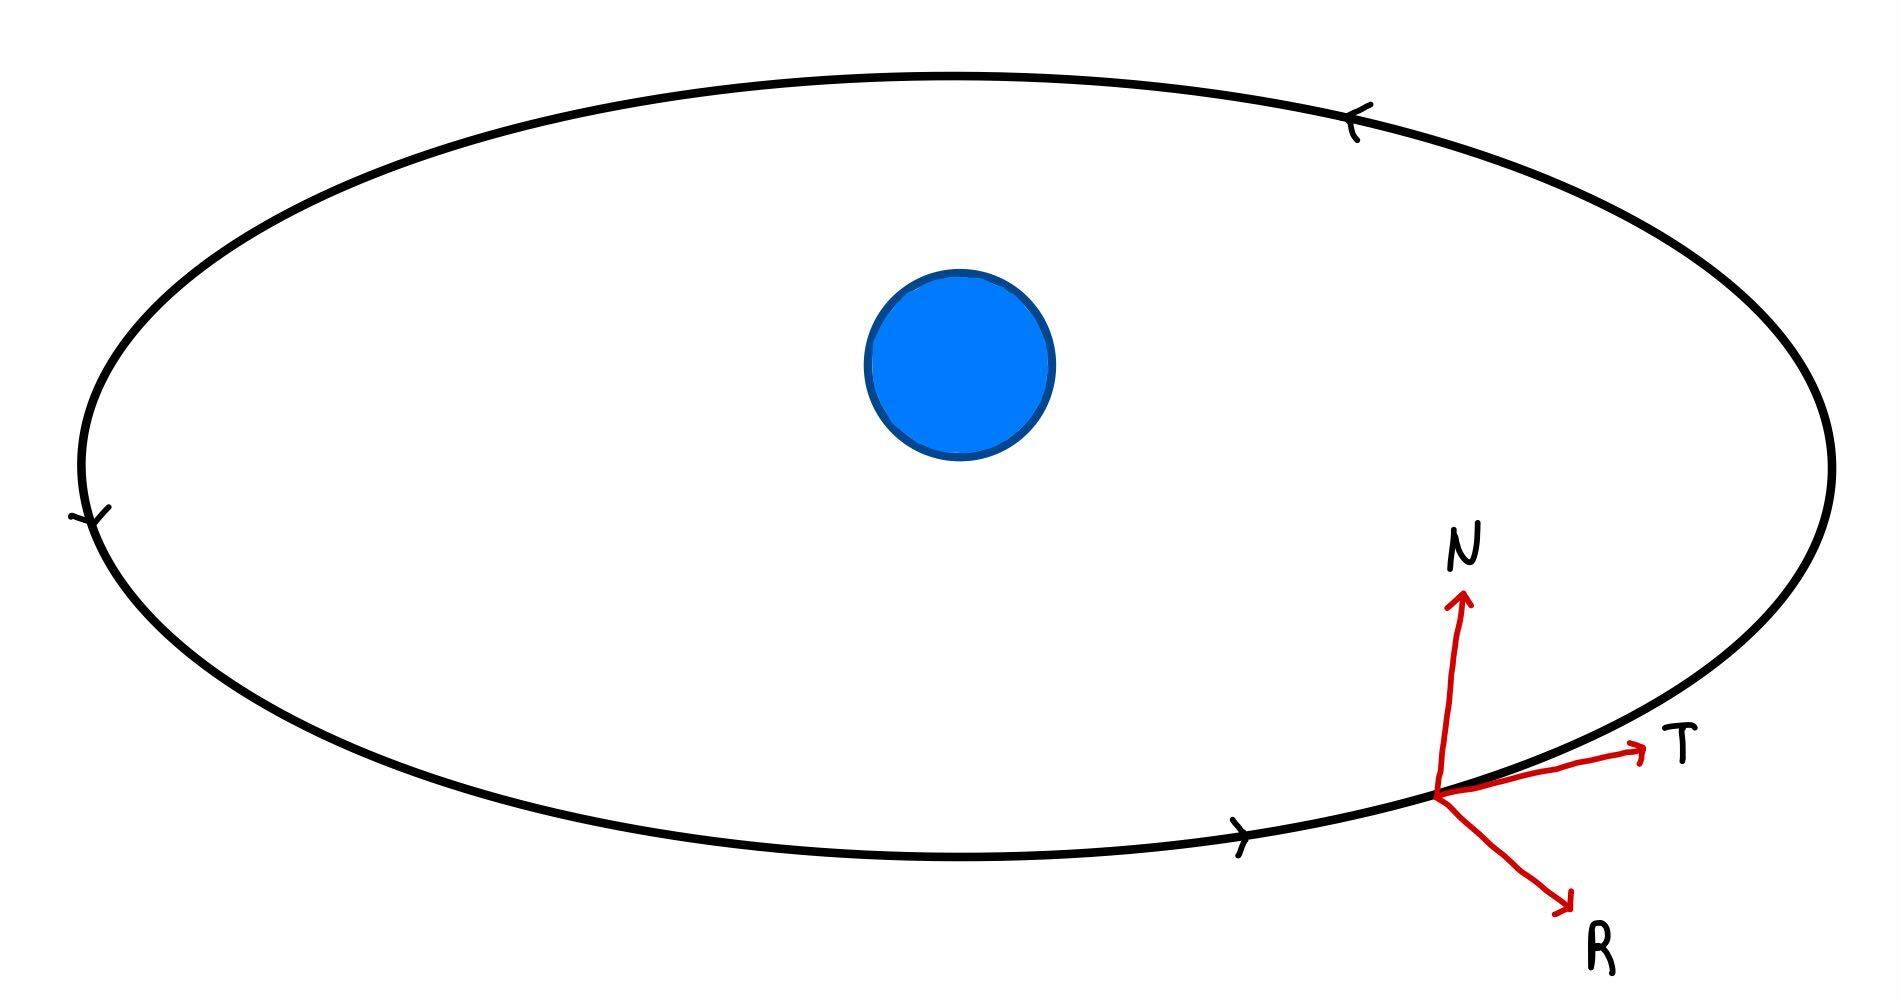
\includegraphics[width=\linewidth]{./figures/rtn-frame.jpg}}
    \caption{Radial-Transverse-Normal (RTN) Coordinate Frame}
    \label{fig:rtn-frame}
\end{figure}

In the context of rendezvous and proximity operations, it is convenient to
identify the the Radial-Transverse-Normal (RTN) coordinate frame centered with
the origin at the center of mass of the target vehicle, as shown in figure
\ref{fig:rtn-frame}. The three axes are aligned in the radial direction, along
the vector from the origin of the center of the earth; the transverse
direction, parallel to the velocity vector, and thus along the orbital path;
and the normal direction, parralel to the orbit's angular momentum vector.

Analyzing the chaser's dynamics and control in the RTN frame has the advantage
of much smaller oscillations in the position-velocity coordinates as
well as conveniently placing out target state at the origin.

Notice that as the target orbits the central body, the RTN frame rotates
relative to the inertial frame of the central body, so the relative position
and dynamics of the chaser is not just a translation from the inertial frame.

We also define our position-velocity (PV) state vector within both the ECI
frame and the RTN frame as $[\vec{x}|\vec{v}]^T=[x,y,z,v_x,v_y,v_z]^T$ with
respect to each frame. Though not the state representation primarily used in
this project, several of the states from the classical orbital elements (COE)
are of import. The full COE state vector is

\begin{equation}
    \label{eq:coes}
    \begin{split}
        e &= \text{Eccentricity} \\
        a &= \text{Semi-major axis (SMA)} \\
        i &= \text{Inclination} \\
        \omega &= \text{Argument of perigee} \\
        \Omega &= \text{Right ascension of the ascending node (RAAN)} \\
        f &= \text{True anomally}
    \end{split}
\end{equation}

For this project, the three important states are: the eccentricity, which is the
eccentricity of our orbit's ellipse; SMA, which (for our
purposes) describes the orbital radius; and the true anomally, which describes,
unlike the other states, where within the orbit we are, rather than the shape
or orientation of the orbit.

%==============================================================================

\subsection{Relative Dynamics}

Within the RTN coordinate frame the following relative dynamics can be derived
\cite{sullivan_comprehensive_2017}:

\begin{equation}
    \label{eq:full-dynamics}
    \begin{split}
        \ddot{x} - 2\dot{f}_c\dot{y} - \ddot{f}_c y - \dot{f}_c^2 x & =
            \frac{-\mu(r_c + x)}{\left[ (r_c+x)^2 + y^2 + z^2\right]^{3/2}} +
            \frac{\mu}{r_c^2} + d_R \\
        \ddot{y} + 2\dot{f}_c\dot{x} + \ddot{f}_c x - \dot{f}_c^2 y & =
            \frac{-\mu y}{\left[ (r_c+x)^2 + y^2 + z^2\right]^{3/2}} + d_T \\
        \ddot{z} & = \frac{-\mu z}{\left[ (r_c+x)^2 + y^2 + z^2\right]^{3/2}} +
            d_N
    \end{split}
\end{equation}

Where $f_c$ is the target's true anomaly, $r_c$ is the target's radius, and
$\vec{d} = [d_R, d_T, d_N]^T$ represents the relative disturbing accelerations
between the target and the chaser in the target's RTN frame.

The first simplifying assumption we make is on the eccentricity of the target's
orbit. If the target's orbit is near circular (the eccentricity is near 0),
then $\dot{f}_c = \text{mean motion} = \sqrt{\frac{\mu}{a^3}}$, where $\mu$ is
the earth's gravitational parameter ($\approx 3.986\cdot10^{14} \text{
m}^2/\text{s}$), and $a$ is the orbit's semi-major axis (SMA). Thus,
$\dot{f}_c$ is constant and $\ddot{f}_c = 0$. In addition, the target's radius
is constant and $r_c = a_c$, where $a_c$ is the target's SMA. This leads to the following
simplified dynamics:

\begin{equation}
    \label{eq:circular-dynamics}
    \begin{split}
        \ddot{x} & =
            -\frac{\mu(r_c + x)}{\left[ (r_c+x)^2 + y^2 + z^2\right]^{3/2}} +
            \frac{\mu}{r_c^2} + 2n\dot{y} + n^2 x + d_R \\
        \ddot{y} & = -\frac{\mu y}{\left[ (r_c+x)^2 + y^2 + z^2\right]^{3/2}} +
            2n\dot{x} + n^2 y + d_T \\
        \ddot{z} & = -\frac{\mu z}{\left[ (r_c+x)^2 + y^2 + z^2\right]^{3/2}} +
            d_N
    \end{split}
\end{equation}

Linearizing this around the target's position, we arrive at the
following linear dynamics known as the Hill-Clohessy-Wiltshire equations \cite{cli_clohessy_nodate}:

\begin{equation}
    \label{eq:linear-dynamics}
    \begin{split}
        \ddot{x} & = 3n^2 x + 2n\dot{y}  + d_R \\
        \ddot{y} & = -2n\dot{x} + d_T \\
        \ddot{z} & = -n^2z + d_N
    \end{split}
\end{equation}

Which we can express in the standard state space form

\begin{equation}
    \label{eq:linear-dynamics-state-space}
    \begin{split}
        \dot{x}_0 &= x_3 \\
        \dot{x}_1 &= x_4 \\
        \dot{x}_2 &= x_5 \\
        \dot{x}_3 &= 3n^2x_0 + 2n x_4 + d_R\\
        \dot{x}_4 &= -2nx_3 + d_T \\
        \dot{x}_5 &= -n^2x_2 + d_N \\
    \end{split}
\end{equation}

%==============================================================================

\subsection{Other Assumptions}

The reality of controlling a spacecraft involves complex actuators, possibly including
electric propulsion, mono-propellant attitude control systems, reaction wheels,
control moment gyros, magnetic torquers, and others that all of their own
dynamics and constraints (such as burn times, thrust profiles, discrete or
continuous thrust levels, etc) that need
to be accounted for in practice. For the purposes of this
project, only the dynamics due to gravity and accelerations in the RTN frame
are considered to simplify the analysis. Therefore, we are neglecting the
attitude control of the chaser and the arrangement (and therefore selection of
thrusters) such that we have have a force in the RTN frame as our only control
input. However in reality, there may be signifcant efficiency gains that can be
realized by considering the arrangement of thrusters when planning maneuvers.

In addition to assumptions on the actuators, we also assume that we have
perfect knowledge of both the target's and chaser's state vector. However,
state estimation for spacecraft is a signifcant challenge, and, depending on
the location (e.g. close enough for relative positioning systems), the uncertainty
in our knowledge can be quite significant.

%==============================================================================
%==============================================================================
%==============================================================================

\section{Simulation}

In order to test the controllers implemented, we created a simulation environment
and several test scenarios to evaluate their performance.

We wrote a restricted two body simulator to propagate the target and chaser
in the ECI frame around Earth. All nonidealities of the orbits, including
oblateness perturbations, solar radiation pressure, lunar perturbations, etc.,
were neglected. Due to the relatively small timescales, distances, and
parameters of the scenarios, these effects would be small, though should not be
ignored in practice.

At every control time step, the chaser's state vector was
converted into a PV vector in the RTN coordinate frame relative to the target.
The simulator saturated the control at 0.01 m/s/s, which is reasonable for the monoprop
thrusters on a relatively small satellite.

The controllers for tracking trajectories were provided a target state at each
control time step, where the target state was generated analytically or read
(and interpolated) from a CSV file depending on the scenario.

\todo{refence to GitHub repo}

%==============================================================================
%==============================================================================
%==============================================================================

\section{Controllers}

%==============================================================================

\subsection{Infinte LQR Linear Controller}

Using the Hill-Clohessy-Wiltshire (\ref{eq:linear-dynamics})
expressed as matrices in state space form, we
implented an infinite LQR controller that solves the following problem:

\begin{equation}
    \label{eq:linear-infinite-lqr}
    \begin{split}
        \min_{x, u} \ \ \  & \frac{1}{2} \int_{t_0}^{\inf} \left( x(t)^T {\bf Q}
            x(t) + u(t)^T {\bf R} u(t) \right)dt \\
        \text{s.t.   } & \dot{x} = {\bf{A}}x + {\bf B}u \\
                     & x(t_0) = x_0
    \end{split}
\end{equation}

Where ${\bf A}$ and ${\bf B}$ are defined as


\begin{equation}
    \label{eq:linearized-state-space}
    \begin{aligned}
        {\bf A} & = \mat{
            0 & 0 & 0 & 1 & 0 & 0 \\
            0 & 0 & 0 & 0 & 1 & 0 \\
            0 & 0 & 0 & 0 & 0 & 1 \\
            3n^2 & 0 & 0 & 0 & 2n & 0 \\
            0 & 0 & 0 & -2n & 0 & 0 \\
            0 & 0 & -n^2 & 0 & 0 & 0 \\
        } \\
        {\bf B} & = \mat{
            0 & 0 & 0 \\
            0 & 0 & 0 \\
            0 & 0 & 0 \\
            1 & 0 & 0 \\
            0 & 1 & 0 \\
            0 & 0 & 1 \\
        }
    \end{aligned}
\end{equation}

and ${\bf Q} = I_{6\times 6}$, ${\bf R} = I_{3\times 3}$. This controller 
stabilizes the chaser in the vicinity of the target. We tested the stabilizing
controller in several scarnios starting it in the vicinity of the target.

\begin{figure}[t]
    \centerline{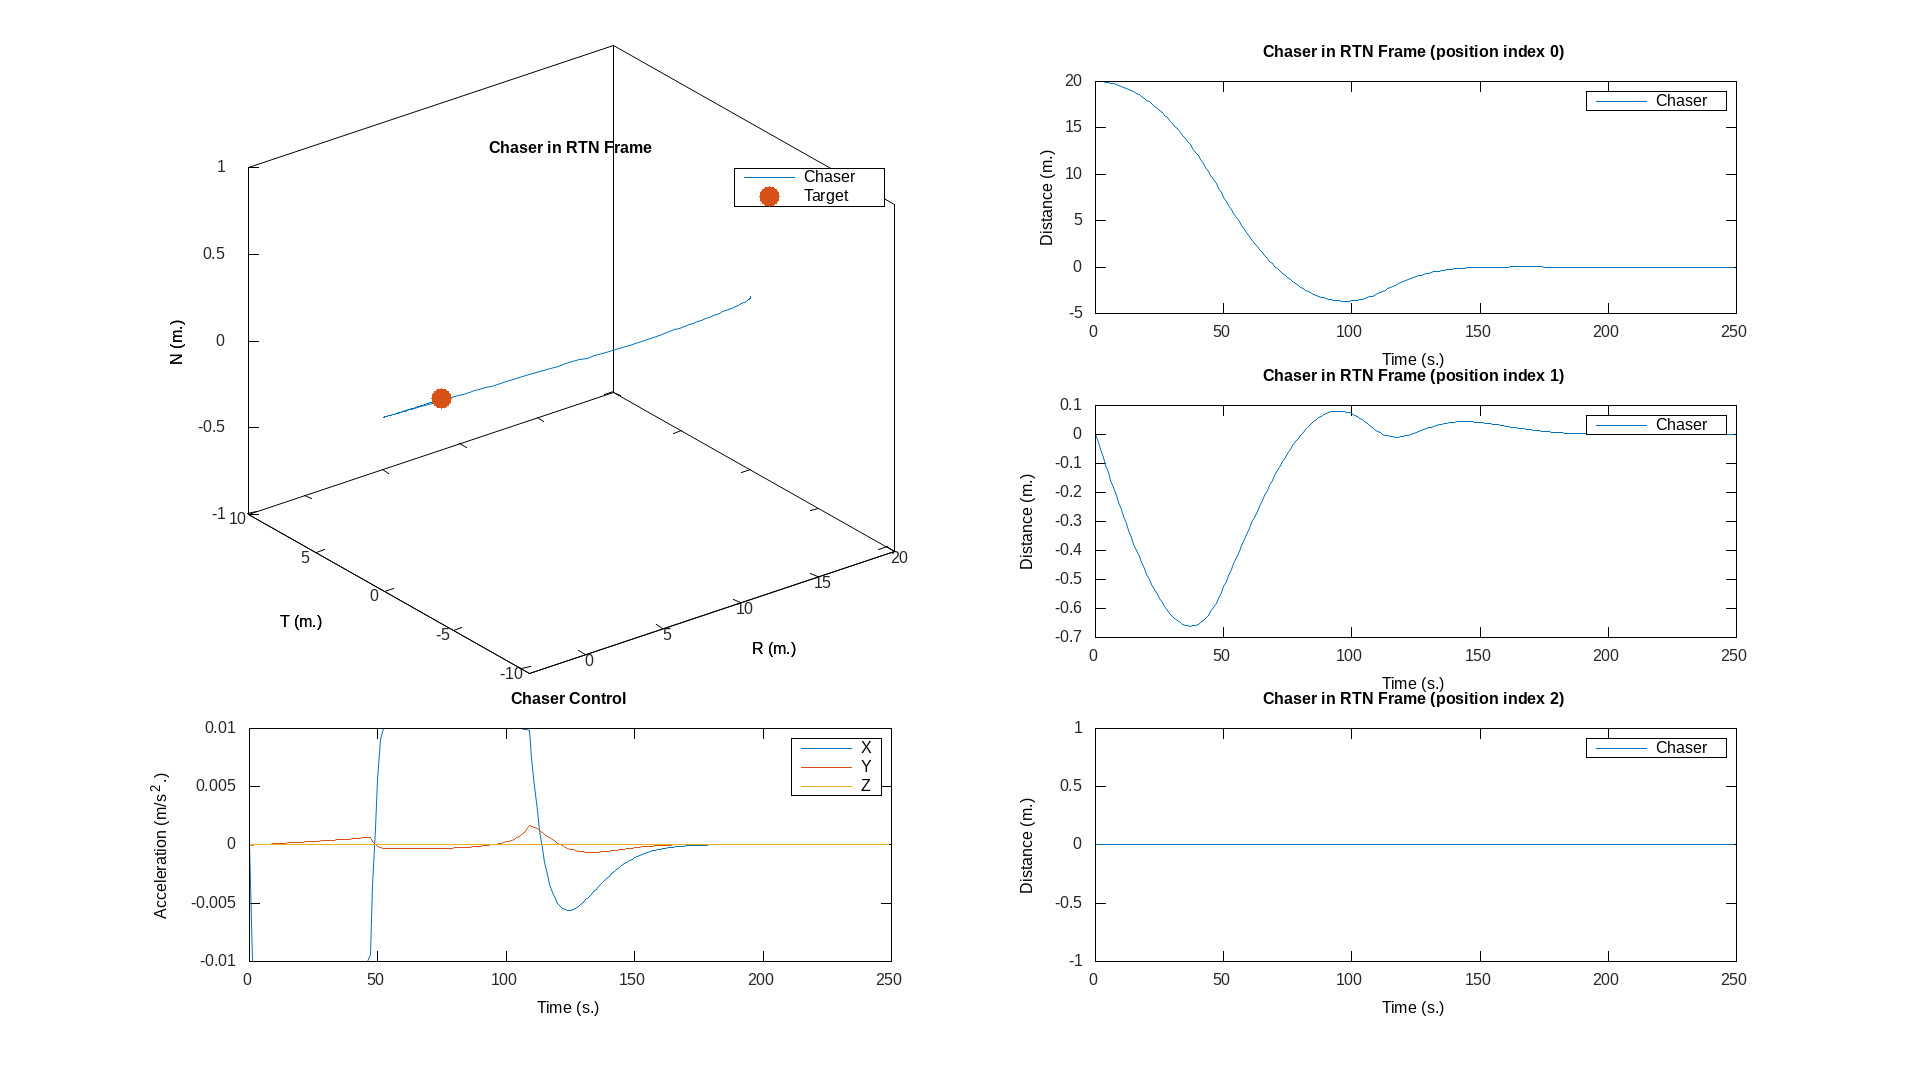
\includegraphics[width=\linewidth]{./figures/simulation_outputs/above20InfiniteLQR-trajStateControl.jpg}}
    \caption{Orbit stabilization starting from 20 meter larger radius.}
    \label{fig:above20}
\end{figure}

\begin{figure}[t]
    \centerline{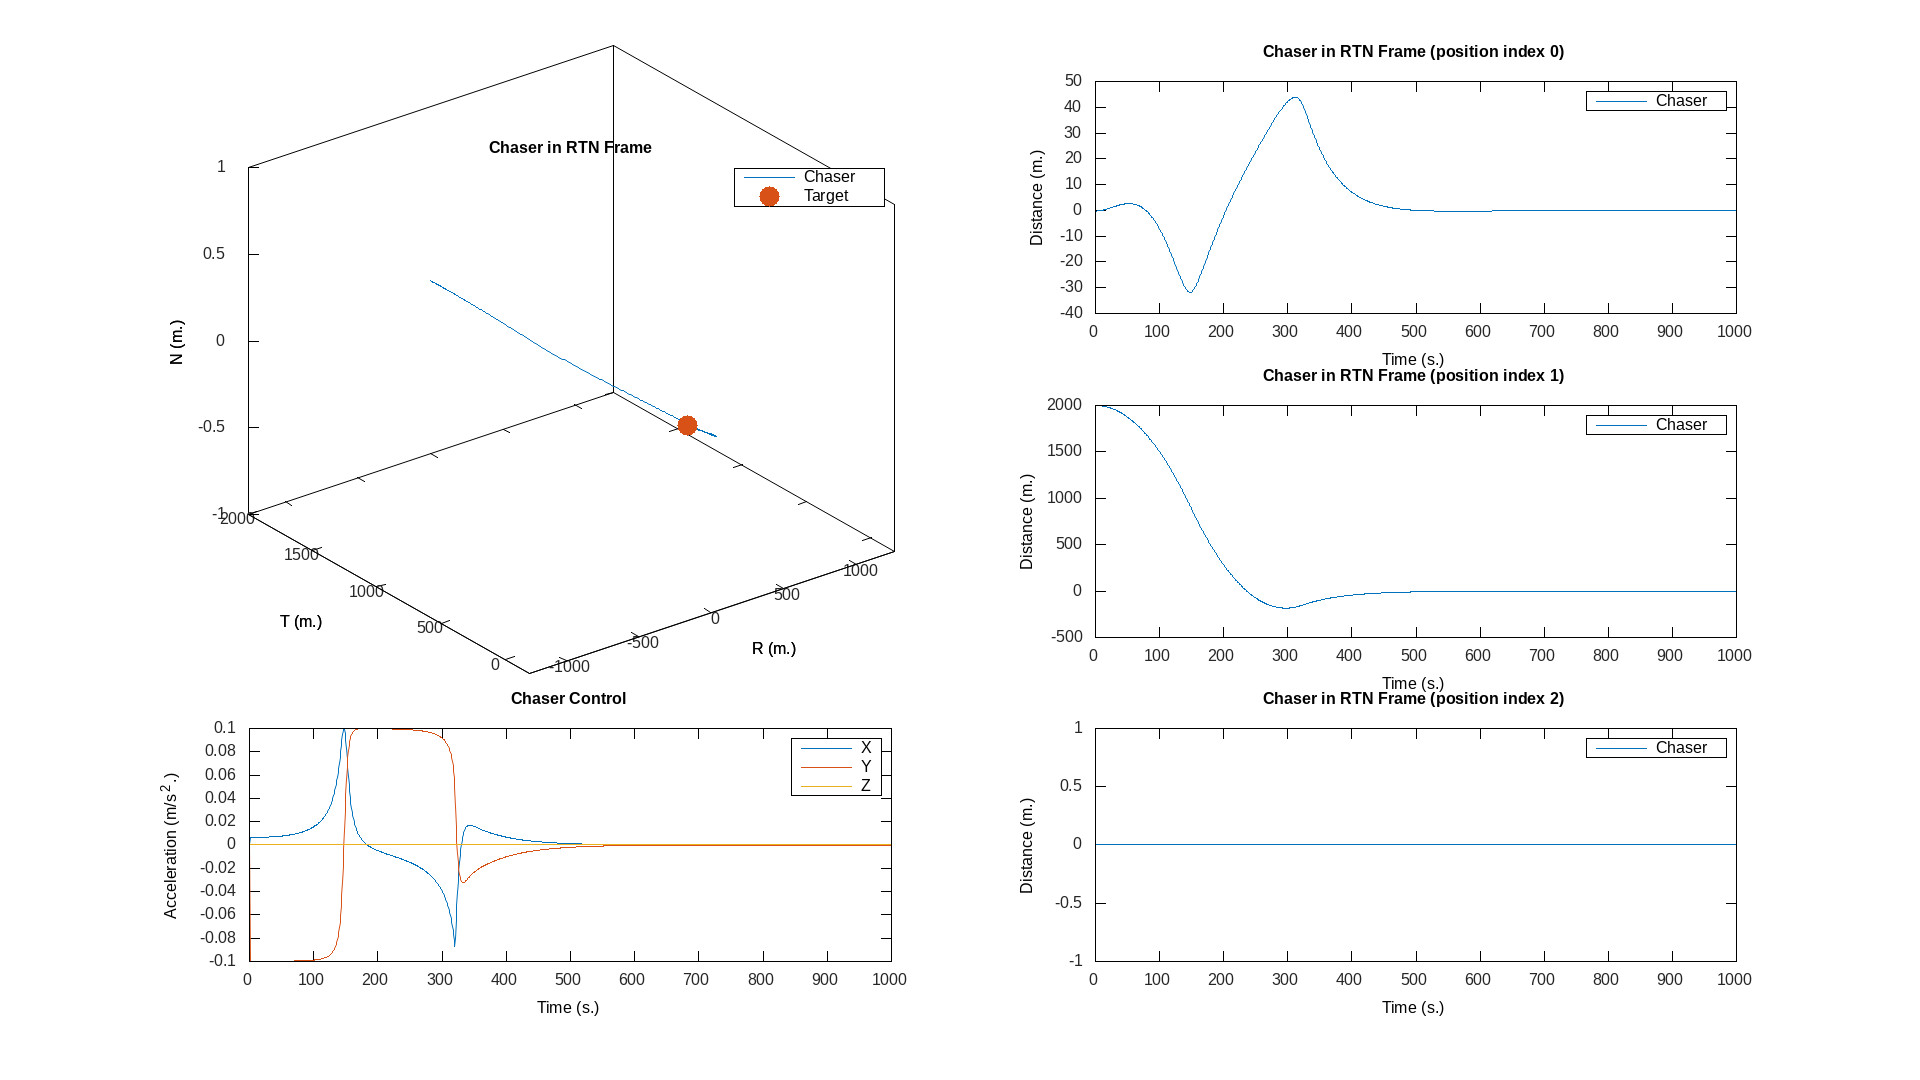
\includegraphics[width=\linewidth]{./figures/simulation_outputs/leading2000InfiniteLQR-trajStateControl.jpg}}
    \caption{Orbit stabilization starting from 2000 meters ahead.}
    \label{fig:leading2000}
\end{figure}

The linear infinite LQR control is able to stabilize the chaser around the
target, though the size of this region of stability appears to be significantly
dependent on the weight matrices Q and R chosen.

For the simulations shown in figures \ref{fig:leading2000} and
\ref{fig:above20} the weight matrices were chosen to be:

\todo{Q and R weight matrices}

These weights were selected by trial and error, but the starting point was
chosen based on the heuristic of weighting $\frac{1}{(\text{error bound})^2}$.

Asside from showing that our dynamics and basic approach work, these
controllers would have little practical use for rendezvous and docking, where
safety constraints on the spacecraft position are very important. Therefore, we
also implemented and tested two trajectory tracking controllers, as discussed
in the next section.

%==============================================================================

\subsection{Infinte LQR Linear Trajectory Tracking Controller}

We also implemented an LQR trajectory tracking controller based on the error
dynamics of the linearized system in (\ref{eq:linear-dynamics}). 
We define the state error $e(t) = x(t) - x_d(t)$, where $x_d$ is our desired
trajectory, and the control error $v(t) = u(t) - u_d(t)$, where $u_d$ is our
desired control. Then the error dynamics are

\begin{equation}
    \label{eq:linearize-error-dynamics}
    \begin{split}
        \dot{e} & = \dot{x} - \dot{x}_d \\
                & = f(x, u) - f(x_d, u_d) \\
                & = f(x_d + e, u_d + v) - f(x_d, u_d) \\
                & = ({\bf A}(x_d + e) + {\bf B}(u_d + v)) - ({\bf A}x_d +
                    {\bf B}u_d) \\
                & = {\bf A}e + {\bf B}v
    \end{split}
\end{equation}

Where ${\bf A}$ and ${\bf B}$ are the same as in
(\ref{eq:linearized-state-space}). Conveniently, the error dynamics of the
linearized system are identical to the dynamics of the linearized system.

Being provided a trajectory to track, one which can be gaurenteed not to
violate any safety constraints, is a more realistic scenario than just an LQR
controller attempting to stabilize the system at the origin.

We tested the trajectory tracking controllers on several 'box' trajectories are
varying orbital radi from Geo Synchronous (~42,000 km) to LEO (~8,000 km).

As the orbit got smaller, the disturbing acceleration required to cancel out
the dyanmics of the system begins to saturate the inputs, causing a loss of
control.

\begin{figure}[t]
    \centerline{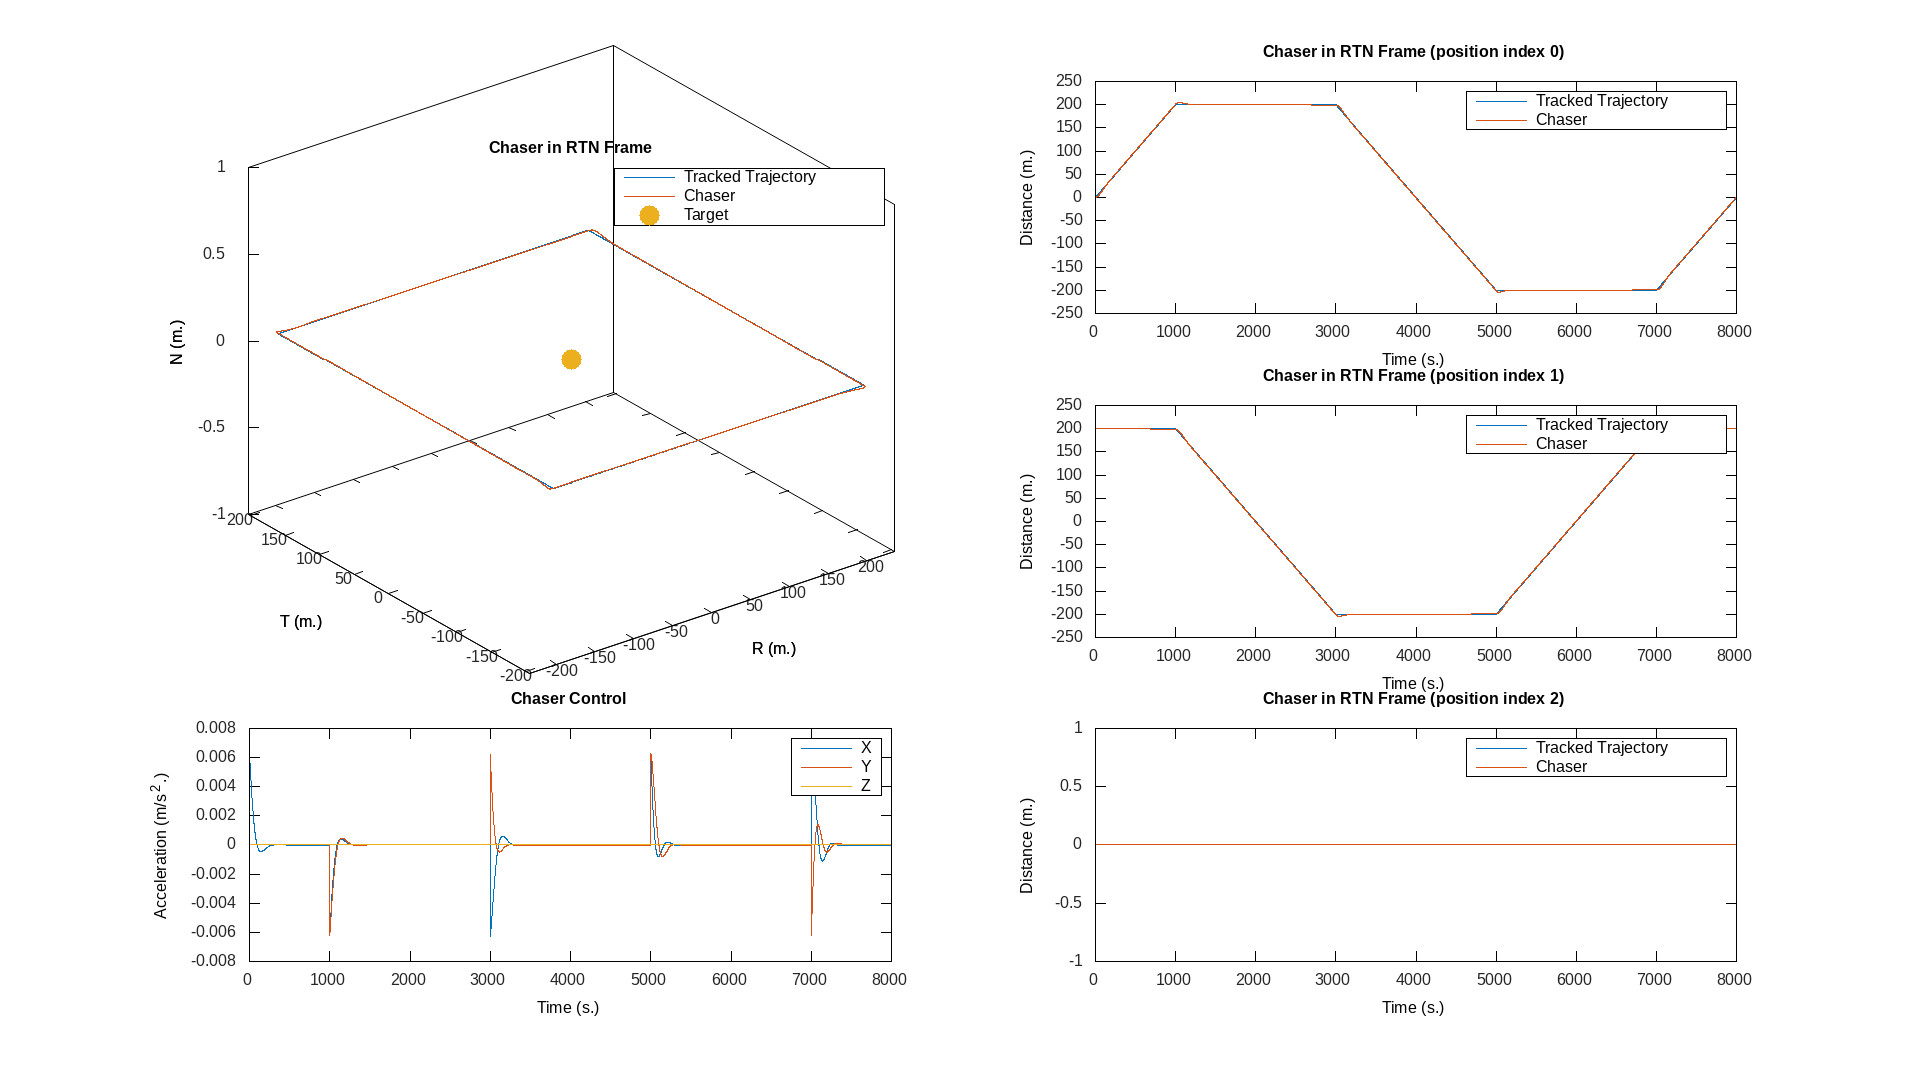
\includegraphics[width=\linewidth]{./figures/simulation_outputs/boxGeoInfiniteLQRLinearTracking-trajStateControl.jpg}}
    \caption{Box trajectory tracking at GEO altitude ($\approx 35000$ km).}
    \label{fig:boxGEO}
\end{figure}

\begin{figure}[t]
    \centerline{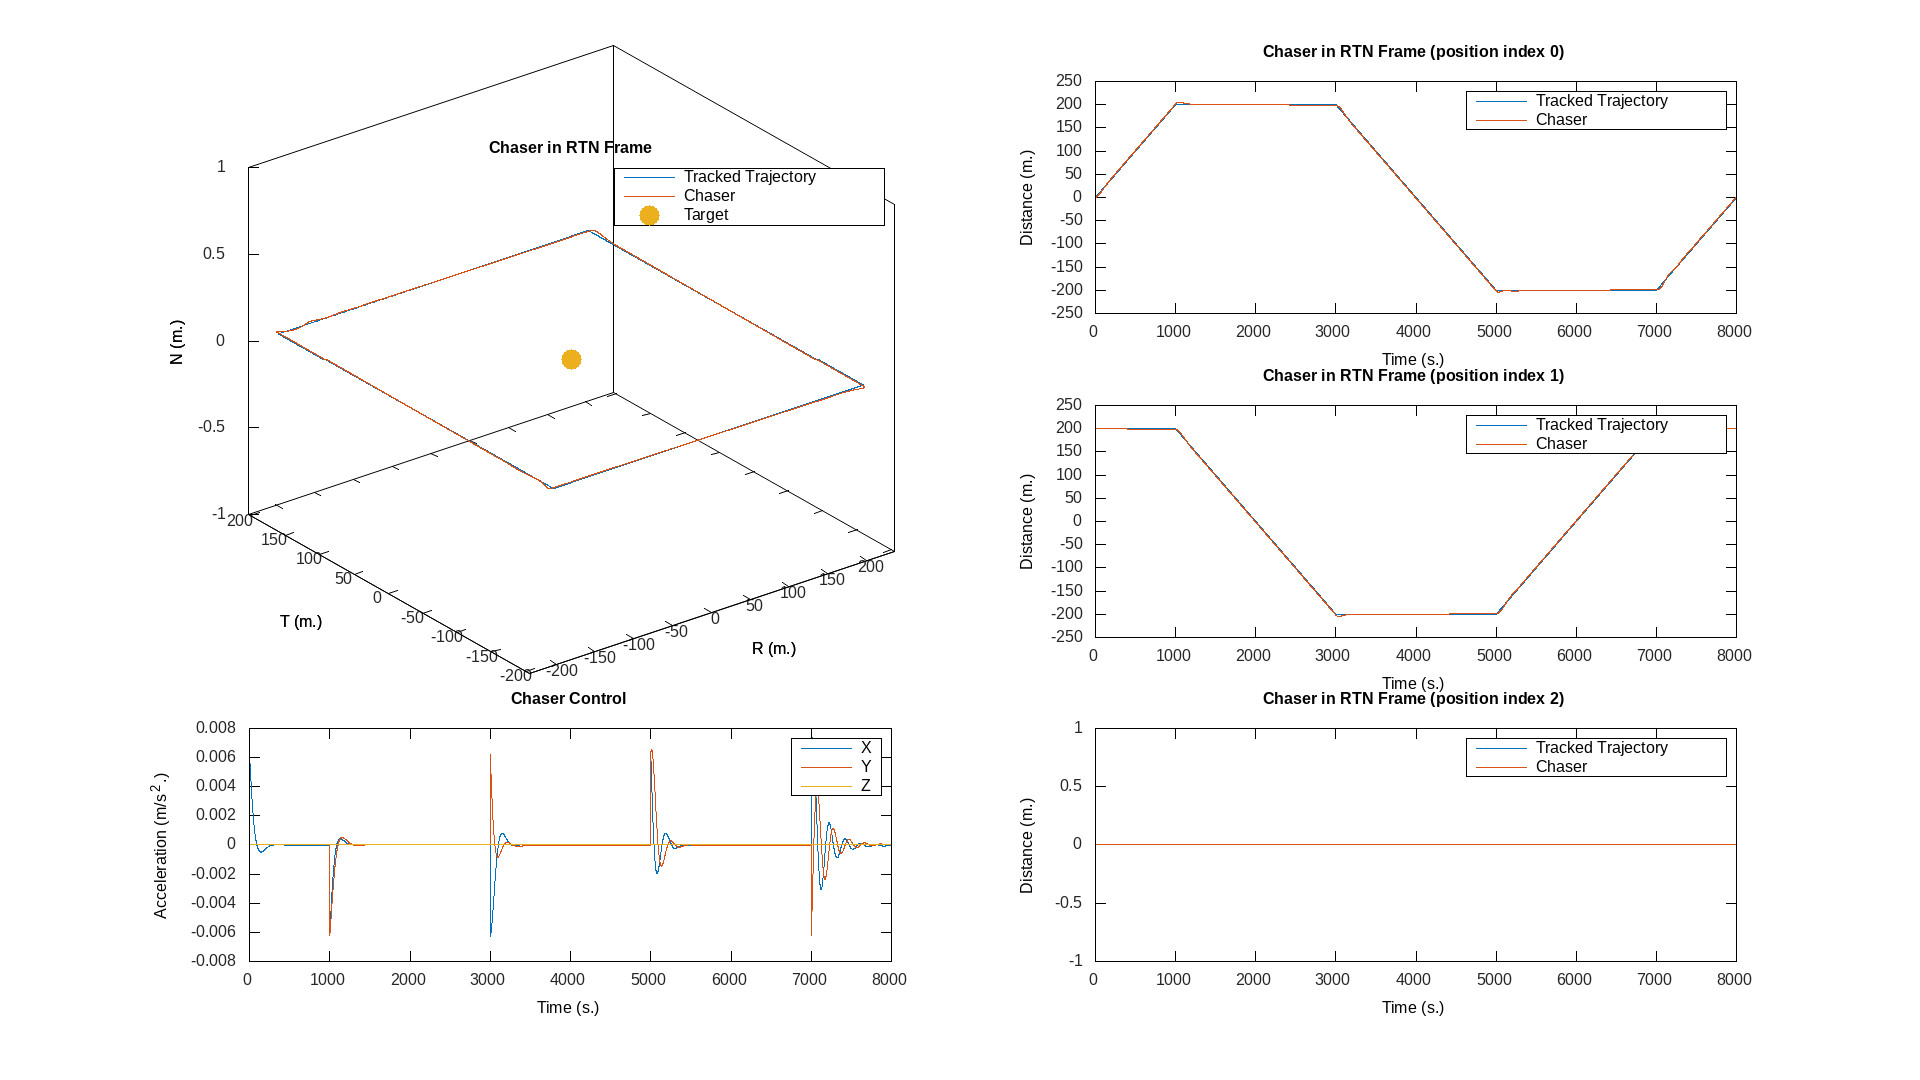
\includegraphics[width=\linewidth]{./figures/simulation_outputs/box30000InfiniteLQRLinearTracking-trajStateControl.jpg}}
    \caption{Box trajectory tracking at 30000 km SMA.}
    \label{fig:box30000}
\end{figure}

\begin{figure}[t]
    \centerline{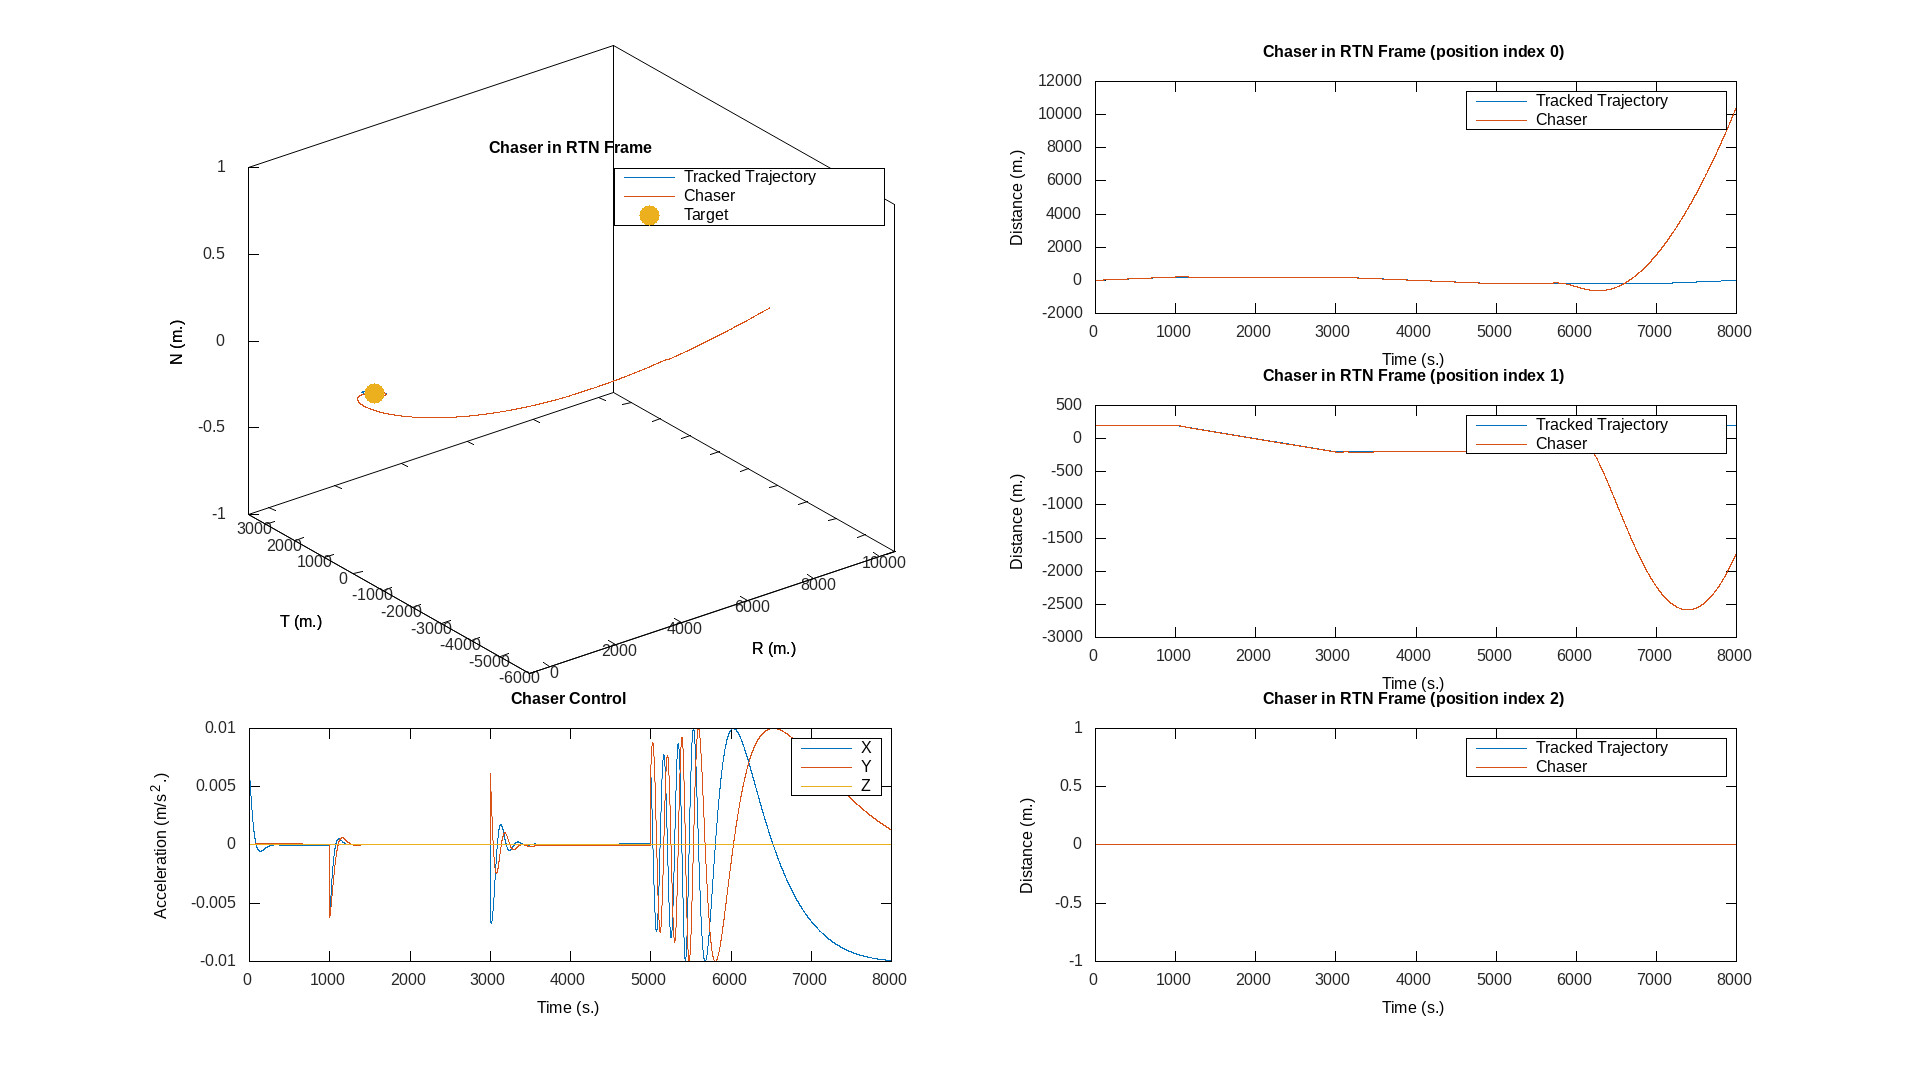
\includegraphics[width=\linewidth]{./figures/simulation_outputs/box20000InfiniteLQRLinearTracking-trajStateControl.jpg}}
    \caption{Box trajectory tracking at 20000 km SMA.}
    \label{fig:box2000}
\end{figure}

%==============================================================================

\subsection{Infinite LQR Time Varying Trajectory Tracking Controller}

We implemnted an LQR trajectory tracking controller based off of the nonlinear
dynamics shown in eq. \ref{eq:circular-dynamics}.

\begin{equation}
    \label{eq:nonlinear-error-dynamics}
    \begin{split}
        \dot{e} & = \dot{x} - \dot{x}_d \\
                & = f(x, u) - f(x_d, u_d) \\
                & = f(x_d + e, u_d + v) - f(x_d, u_d) \\
                & = F(e, v, x_d(t), u_d(t))
    \end{split}
\end{equation}

The time varying linearized error dynamics are then given by

\begin{equation}
    \label{eq:nonlinear-error-dynamics-lvi}
    \dot{e} = {\bf A}(t)e + {\bf B}(t)v
\end{equation}

where

\begin{equation}
    \label{eq:ltvA}
    \begin{aligned}
        {\bf A}(t) &= \frac{\partial F}{\partial e}|_{x_d(t),u_d(t)}
    \end{aligned}
\end{equation}

\begin{equation}
    \label{eq:ltvB}
    \begin{aligned}
        {\bf B}(t) &= \frac{\partial F}{\partial v}|_{x_d(t),u_d(t)}
    \end{aligned}
\end{equation}

Rather than performing the deirvation by hand, we used the symbolic mathematics
library SymEngine \todo{ref SymEngine} to derive the symbolic matrices for
${\bf A}(t)$ and ${\bf B}(t)$. From the symbolic matrices, we performed code
generation at runtime to create a function for each symbolic matrix that, given
a vector of the desired state and control, returned ${\bf A}$ and ${\bf B}$.
The generated code was compiled to a shared object and then loaded into memory
and the function pointers retrieved.

%==============================================================================
%==============================================================================
%==============================================================================

\section{Extensions}

There are many extensions and variations on the system and the controllers that
could be taken. Of signifcant interest to myself, is extending the LTV
controller to the noncircular case, where the first and second time derivatives
of the true anomally come into the system. This would enable the controllers to
function in a larger vicinity of the target, as well in elliptical orbits.

Similiarly, it would be interesting to extend the simulation and controllers to
the restricted three body problem involving the earth, moon, and spacecraft. Of
particular interest, would be rendezvous and proximity operations in Near
Rectilinear Halo Orbits about the Moon (these are extremely elliptical lunar
orbits that verge on being closer to L2 halo orbits than lunar orbits) where
the planned NASA Gateway manned space station will be.

\bibliography{mybibfile}
\bibliographystyle{plain}

\end{document}
